\documentclass[11pt]{article}

\usepackage[margin=1in]{geometry}
\usepackage[T1]{fontenc}
\usepackage[utf8]{inputenc}
\usepackage{lmodern}
\usepackage{microtype}
\usepackage{amsmath, amssymb, amsfonts}
\usepackage{bm}
\usepackage{graphicx}
\usepackage{booktabs}
\usepackage{multirow}
\usepackage{xcolor}
\usepackage{hyperref}
\usepackage[nameinlink,capitalise]{cleveref}
\usepackage{enumitem}

\hypersetup{
  colorlinks=true,
  linkcolor=blue!50!black,
  citecolor=blue!50!black,
  urlcolor=blue!50!black
}

\title{Layer-Depth Attention Routing in Transformers}
\author{}
\date{}

\begin{document}
\maketitle

\begin{abstract}
Transformers propagate information effectively along the token dimension, but access to intermediate representations formed at earlier layers remains indirect. We study whether a token at the current layer can benefit from directly reading its own depth history, rather than relying only on repeated residual propagation through the stack. To this end, we introduce a layer-depth attention routing mechanism that augments standard self-attention with a same-position cross-layer memory branch. In this paper, we instantiate and evaluate this idea in decoder-only language models. The current implementation uses a single shared query for row-wise token attention and depth-wise memory retrieval, stores sublayer-level history, and archives historical memory through projected keys and values. On WikiText-103, across multiple settings including 8-layer and 16-layer models, different sequence lengths, and long training budgets, the method consistently improves perplexity over strong Transformer baselines by roughly 2\% to 4\%. Additional attention-allocation analysis shows that deeper layers assign substantial attention mass to the depth branch and selectively retrieve a small number of high-value early-layer memory slots, rather than ignoring the added pathway. These results indicate that explicit depth history is a useful information source even for already strong decoder baselines, while also revealing a clear trade-off: the current prototype incurs noticeable runtime overhead. Overall, the results position layer-depth attention routing as a stable and promising architectural direction for Transformer language models, while leaving memory-path optimization and stronger memory parametrization studies to future work.
\end{abstract}

\section{Introduction}

Transformer language models are built around token-wise attention, where each layer reads contextual information from other positions in the sequence. A useful way to interpret this architecture is as a two-dimensional computation graph over token positions and layer depth. Under this view, recurrent models mainly propagate information through chained local transitions, while self-attention dramatically shortens communication along the token axis by allowing a token to directly access its prefix within one layer. However, the same perspective also reveals a remaining asymmetry: intermediate representations formed by the same token at earlier layers are still only indirectly accessible in standard decoder-only Transformers.

Residual connections do provide a depth-wise transmission path, so standard Transformers are not entirely lacking in cross-layer communication. But this path is uniform and additive rather than selective: earlier-layer information is mixed forward through the residual stream, not explicitly retrieved on demand for the current token. As depth increases, useful earlier-layer signals may therefore be diluted among many subsequent transformations. This observation motivates a simple question: can a decoder-only language model improve by augmenting token attention with a direct layer-depth memory branch? If the current token could jointly attend to both the usual row-wise prefix context and its own cross-layer history, then the model might reuse partially refined intermediate states more effectively instead of repeatedly reconstructing them through the stack.

In this work, we study this question through a controlled family of cross-layer memory mechanisms for decoder-only Transformers. Our final design uses a single query to route both row-wise token attention and depth-wise memory retrieval, stores memory at the sublayer level, and archives historical states through projected keys and values. The resulting mechanism extends each attention step from pure token interaction to a joint token-depth routing problem. In the computation-graph view, the method preserves the short communication path along the token axis while introducing a more direct and selective access path along the depth axis.

The resulting gains are not dramatic, but they are stable. Across multiple WikiText-103 settings, including 8-layer and 16-layer models, different sequence lengths, and long training budgets, the proposed method consistently improves perplexity over strong Transformer baselines by roughly 2\% to 4\%. At the same time, the method introduces nontrivial runtime overhead, and the measured slowdown is larger than the pure theoretical compute gap, indicating that the current prototype implementation is not yet fully optimized.

These results support a restrained but meaningful conclusion: explicit depth-history access is useful for decoder-only language modeling, and it can yield repeatable improvements even on already strong baselines. However, the method is best viewed as a promising architectural direction rather than a fully optimized replacement for standard self-attention.

\paragraph{Contributions.}
This paper makes the following contributions:
\begin{enumerate}[leftmargin=1.5em]
    \item We formulate decoder-only attention as a \textbf{joint row-depth routing problem}, where the current token can read both prefix tokens and its own cross-layer history.
    \item We introduce a practical final design based on \textbf{single-query routing, sublayer memory, and projected historical K/V}, and show that this combination gives the most stable results among the tested variants.
    \item We show on WikiText-103 that the method yields \textbf{consistent 2\% to 4\% perplexity improvements} across multiple settings, including 8-layer and 16-layer models and different sequence lengths.
    \item We provide \textbf{attention-allocation evidence} showing that the depth branch is actively used in middle and late layers and that retrieval concentrates on a small number of high-value historical slots rather than collapsing to uniform mixing.
    \item We analyze the method's cost and show that while the theoretical extra compute is moderate, the current prototype incurs additional systems-level overhead, highlighting an important optimization direction for future work.
\end{enumerate}

\section{Method}

\subsection{Problem Setup}

Consider a decoder-only Transformer with $L$ layers. At layer $l$, the hidden state at token position $t$ is denoted by $x_t^{(l)}$. Standard causal self-attention allows $x_t^{(l)}$ to read row-wise context from the prefix positions $\{1, \dots, t\}$ in the same layer. However, it does not explicitly expose the cross-layer history $\{x_t^{(1)}, \dots, x_t^{(l-1)}\}$ for direct retrieval.

We aim to augment standard self-attention with a depth-memory branch that allows the current token to retrieve same-position information formed at previous layers.

More generally, we view the model as a directed computation graph whose nodes are hidden states $x_t^{(l)}$. The communication distance between two states is the minimum number of graph edges required for one state to influence the other. Under this view, standard causal self-attention already shortens token-wise communication distance, since a token can directly access its full prefix within one layer. Our objective is to similarly shorten access to same-position earlier-layer states, which in the standard decoder are otherwise reached mainly through residual mixing across successive layers.

\subsection{Row Attention and Depth Memory}

For each layer, we keep the usual row-wise token attention branch over the current sequence. In parallel, we maintain a depth-memory archive consisting of same-position history from earlier layers or sublayers. The current token then produces a single query that is used for two routing decisions:
\begin{itemize}[leftmargin=1.5em]
    \item row-wise routing over current-layer prefix tokens;
    \item depth-wise routing over same-position historical memory.
\end{itemize}
The row branch and depth branch produce scores that are concatenated and normalized jointly, so the model allocates attention mass across both sources within one competition space.

\subsection{Final Design Used in This Paper}

The final method has three defining design choices.

\paragraph{Single-Q.}
The same query representation is used for both row attention and depth-memory lookup. This avoids introducing an additional query branch and gives a simpler routing mechanism than dual-query variants.

\paragraph{Sublayer Memory.}
Instead of storing only one memory item per Transformer block, we cache history at the sublayer level. In the current implementation, this means that attention-side and FFN-side intermediate states can both contribute memory entries. This produces a richer depth archive than block-only storage.

\paragraph{Projected K/V.}
Historical memory is archived through projected keys and values rather than leaving it in raw hidden-state form. This gives the current layer a learned memory space for matching and aggregation, and empirically performs more stably than removing projection entirely.

\subsection{Layer Computation}

At layer $l$, let the current hidden sequence be
\[
X^{(l)} \in \mathbb{R}^{B \times S \times D}.
\]
The row-attention branch first computes a fused token-attention projection:
\[
[Q_{\text{row}}, K_{\text{row}}, V_{\text{row}}] = W_{\text{qkv}} X^{(l)}.
\]
After reshaping into multi-head form, the model computes the standard causal token-attention scores over prefix positions:
\[
A_{\text{row}} = \frac{Q_{\text{row}} K_{\text{row}}^\top}{\sqrt{d}}.
\]

For the depth-memory branch, the final design uses the same query as the row branch:
\[
Q_{\text{depth}} = Q_{\text{row}}.
\]
The memory archive is built from previously produced sublayer states. In the current implementation, each block contributes multiple same-position memory entries, so the archive for layer $l$ contains projected historical keys and values from earlier layers and earlier sublayers:
\[
\mathcal{M}^{(l)} = \{(K_{\text{mem}}^{(1)}, V_{\text{mem}}^{(1)}), \ldots, (K_{\text{mem}}^{(m)}, V_{\text{mem}}^{(m)})\}.
\]
Each historical entry is archived through learned projections:
\[
K_{\text{mem}} = W_k^{\text{mem}} H,\qquad V_{\text{mem}} = W_v^{\text{mem}} H,
\]
where $H$ denotes the corresponding sublayer hidden state. In the current implementation, the memory projection matrices are shared across layers, so the historical archive is parameterized by global memory projections rather than separate per-layer memory heads.

Given the memory archive, the current layer computes depth-memory scores by matching the current token query against the historical same-position keys:
\[
A_{\text{depth}} = \frac{Q_{\text{depth}} \cdot K_{\text{mem}}}{\sqrt{d}}.
\]
The key design choice is that row-wise token scores and depth-wise memory scores are concatenated and normalized jointly:
\[
A = [A_{\text{row}}; A_{\text{depth}}],\qquad P = \operatorname{softmax}(A).
\]
This means the model does not make two independent attention decisions. Instead, it allocates one unified attention budget across two competing sources:
\begin{itemize}[leftmargin=1.5em]
    \item current-layer token context;
    \item historical same-position depth memory.
\end{itemize}
The final output context is then the sum of the row-context aggregation and the memory-context aggregation:
\[
O = O_{\text{row}} + O_{\text{depth}}.
\]
The resulting sequence is passed through the usual output projection and then through the remaining residual/FFN components of the Transformer block. \Cref{fig:architecture} summarizes the resulting block structure.

\begin{figure}[t]
    \centering
    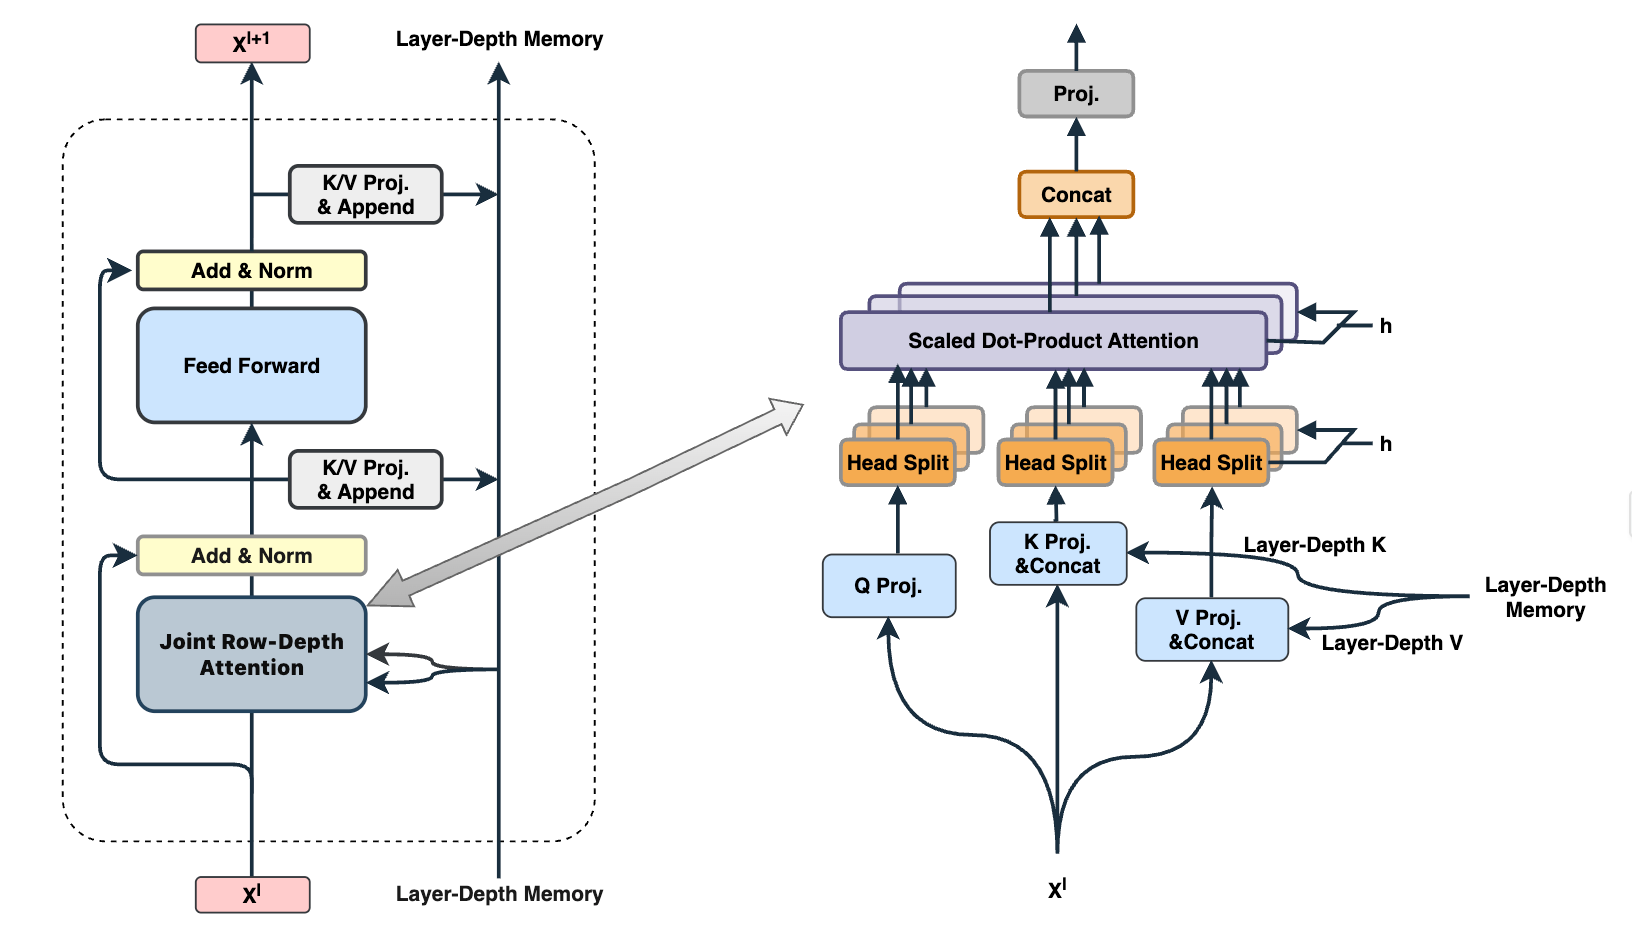
\includegraphics[width=0.95\linewidth]{figures/figure1_architecture.png}
    \caption{Overview of the proposed layer-depth attention routing block. The standard row-wise causal attention pathway is preserved, while the block also exports sublayer-level K/V entries to a layer-depth memory archive. At the next layer, the current token uses a single query to route attention jointly over current-layer token context and earlier-layer same-position memory. Row-wise scores and depth-memory scores are concatenated before a shared softmax, so both sources compete for one unified attention budget.}
    \label{fig:architecture}
\end{figure}

\subsection{Complexity and Memory Overhead}

For a decoder-only Transformer layer with hidden width $D$, sequence length $S$, batch size $B$, and MLP ratio $r$, a standard baseline layer has the following leading-order cost:
\[
C_{\text{base, layer}} = (4 + 2r)BSD^2 + 2BS^2D.
\]
For the commonly used $r = 4$ setting, this becomes:
\[
C_{\text{base, layer}} = 12BSD^2 + 2BS^2D.
\]

Relative to the baseline, the proposed method adds three kinds of work. First, each layer must build the memory archive entries that will be consumed by later layers. In the final projected-memory design, this introduces extra memory-side K/V projections on top of the usual row-attention projections. Second, each layer performs depth-memory matching in addition to standard token-token attention. Third, the sublayer-memory design increases the number of archived entries, because attention-side and FFN-side intermediate states can both contribute to the history bank.

Under this approximation, the final method has leading-order per-layer cost
\[
C_{\text{method, layer}} \approx (8 + 2r)BSD^2 + 2BS^2D + 2BSM_iD,
\]
where $M_i$ denotes the number of historical memory entries visible to layer $i$. For the current $r = 4$ setting,
\[
C_{\text{method, layer}} \approx 16BSD^2 + 2BS^2D + 2BSM_iD.
\]

The important point is that the extra cost comes from two sources:
\begin{itemize}[leftmargin=1.5em]
    \item extra learned projection work, which scales with $BSD^2$;
    \item extra memory matching and aggregation, which scales with $BSM_iD$.
\end{itemize}

Theoretical MAC analysis suggests that the final method should be moderately more expensive than the baseline, but not by the full amount observed in end-to-end runtime. In our current implementation, the measured wall-clock slowdown is larger than the pure analytical compute ratio. This strongly suggests that the current prototype still pays additional systems-level overhead beyond the method's unavoidable arithmetic cost.

\section{Experiments}

\subsection{Benchmark and Setup}

Our main benchmark is \textbf{WikiText-103} in the raw-text setting. All experiments use a BPE tokenizer, specifically the GPT-2 tokenizer, and train decoder-only language models with tied input/output embeddings unless otherwise noted.

All models in the main comparison use the same decoder-only Transformer backbone family implemented in \texttt{ablation\_models.py}. Unless a specific ablation changes the attention mechanism itself, the backbone remains matched across methods in hidden size, head count, MLP ratio, positional embeddings, and language-model head structure.

The main completed result pool already supports a coherent comparison across multiple settings:
\begin{itemize}[leftmargin=1.5em]
    \item 8-layer, $seq\_len=256$, $40000$ and $80000$ steps;
    \item 16-layer, $seq\_len=256$, $80000$ steps;
    \item 8-layer, $seq\_len=512$, $80000$ steps;
    \item projected-K/V versus non-projected historical K/V.
\end{itemize}
Most runs use $d\_model=384$, $num\_heads=8$, $mlp\_ratio=4$, tied embeddings, and learned positional embeddings.

Validation is performed periodically during training, while the test set is evaluated only at the end of the run. For this reason, we consistently report \textbf{Best Val PPL} and \textbf{Final Test PPL} rather than best test perplexity.

\subsection{Main Results}

Across all completed settings, the final \textbf{single-q + sublayer + projected K/V} method consistently outperforms the standard Transformer baseline in both best validation perplexity and final test perplexity.

In the 8-layer, $seq\_len=256$ setting, the method reduces final test perplexity from $34.53$ to $33.53$ at $40000$ steps, and from $28.47$ to $27.58$ at $80000$ steps. In the 16-layer, $seq\_len=256$ setting, it further reduces final test perplexity from $26.28$ to $25.55$. The gain also persists at longer context length, where the 8-layer, $seq\_len=512$ setting improves from $24.03$ to $23.46$.

Taken together, the currently completed settings show stable relative final-test-perplexity improvements of roughly 2.3\% to 3.1\% across model depth, context length, and training budget. Although the absolute gains are moderate rather than dramatic, they are consistent across all currently completed main settings.

\subsection{Attention Allocation and Retrieval Patterns}

Beyond perplexity, the attention analyses provide direct evidence that the added depth branch is functionally active rather than a passive architectural perturbation. The most basic statistic is the average attention mass assigned to the row branch versus the depth branch. In the 16-layer sublayer-memory model, early layers remain dominated by row-wise token attention, but middle and late layers allocate substantially more mass to depth retrieval; in the deepest layers, the average depth mass becomes comparable to or slightly larger than the row mass.

This raw layer-wise increase must be interpreted carefully. Deeper layers also expose more memory slots, so part of the increase in total depth mass is structurally induced by a larger candidate set. We therefore also inspect slot-normalized views and the depth-slot heatmap. These show that the growth in total depth usage is only partly explained by slot count: even after accounting for the number of available historical slots, middle and late layers still retain nontrivial per-slot depth usage. More importantly, the slot-allocation heatmap shows that the model does not distribute attention uniformly over all available history. Instead, it exhibits a marked preference for a small set of early memory slots, especially those near the bottom of the network.

The single-example attention matrices clarify the qualitative difference between the baseline and the proposed method. In the baseline, the entire attention budget is distributed over token positions only. In the proposed model, the row branch is preserved, but the joint matrix additionally assigns visible mass to a separate region of depth slots. This makes the final attention pattern more selective: the model is no longer limited to distributing mass across token positions alone, and instead routes part of the budget toward a small number of high-value historical states.

\begin{figure}[t]
    \centering
    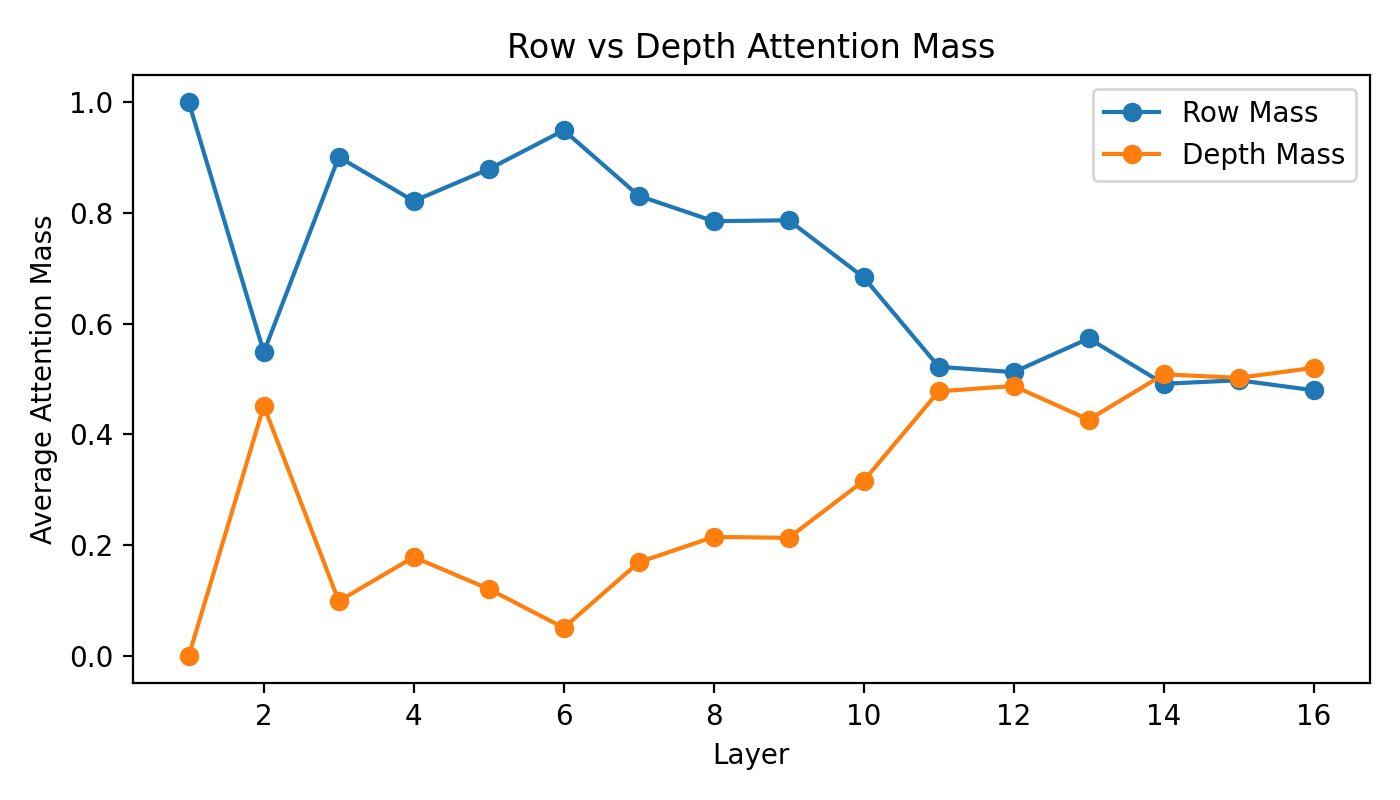
\includegraphics[width=0.48\linewidth]{figures/figure3a_row_vs_depth_mass.png}\hfill
    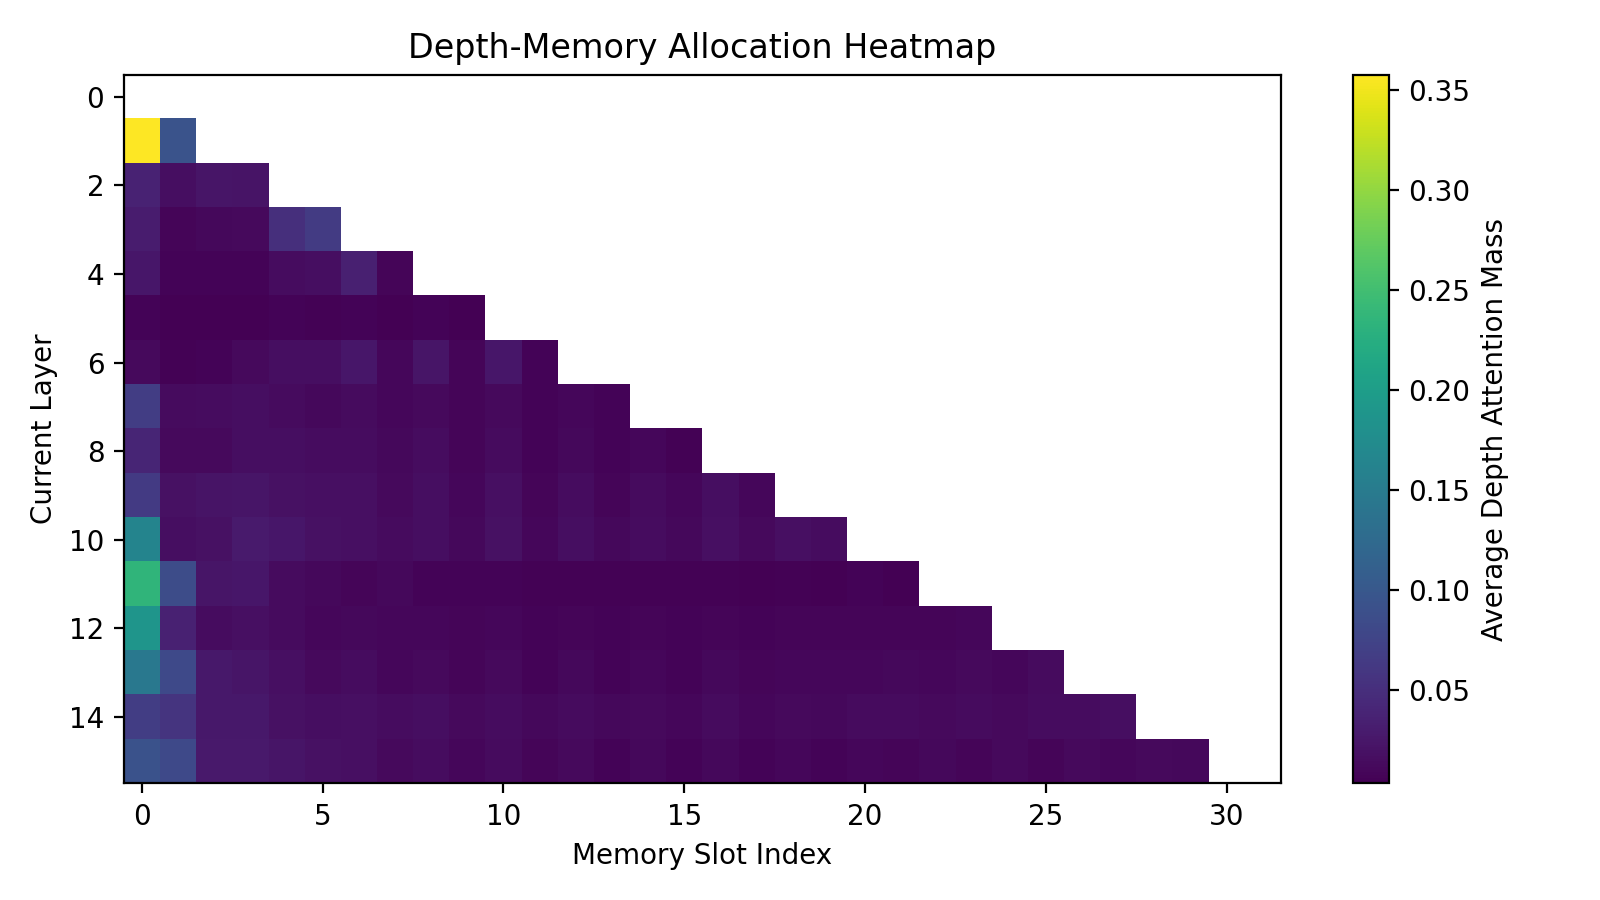
\includegraphics[width=0.48\linewidth]{figures/figure3b_depth_slot_heatmap.png}

    \vspace{0.8em}

    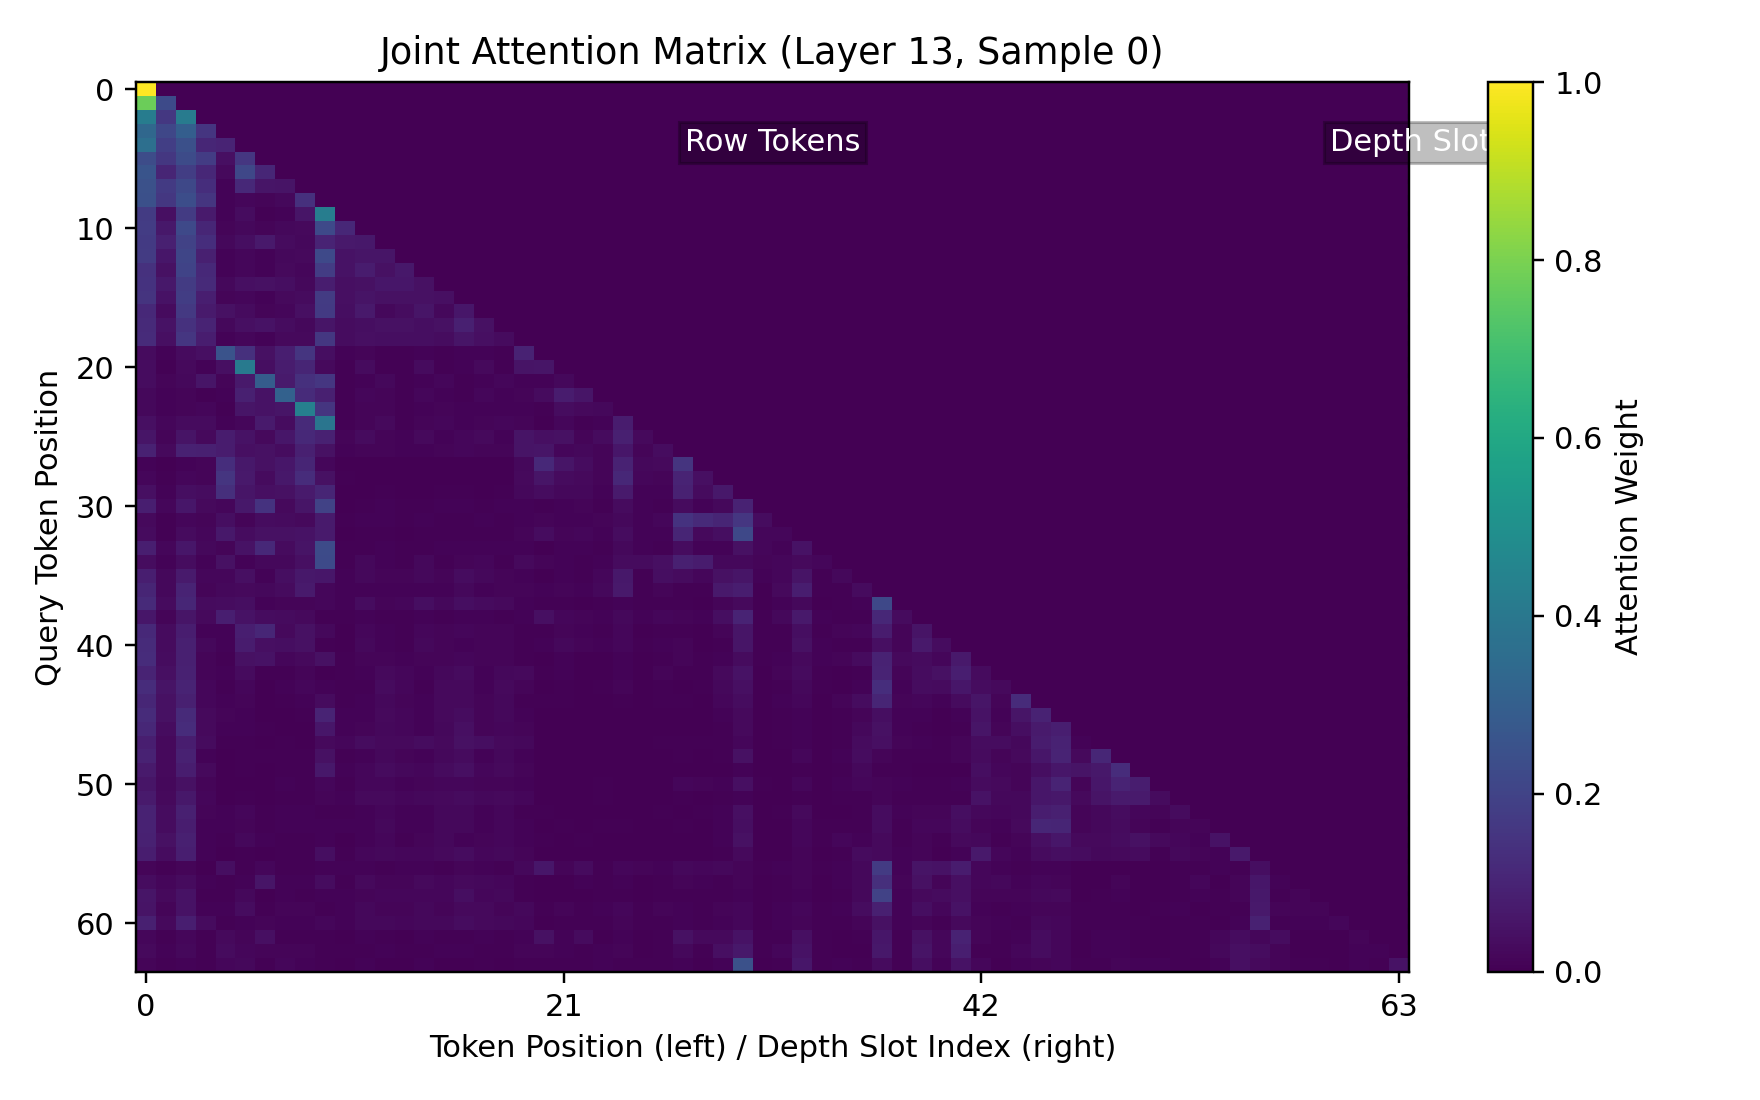
\includegraphics[width=0.48\linewidth]{figures/figure3c_baseline_joint_attention_s64.png}\hfill
    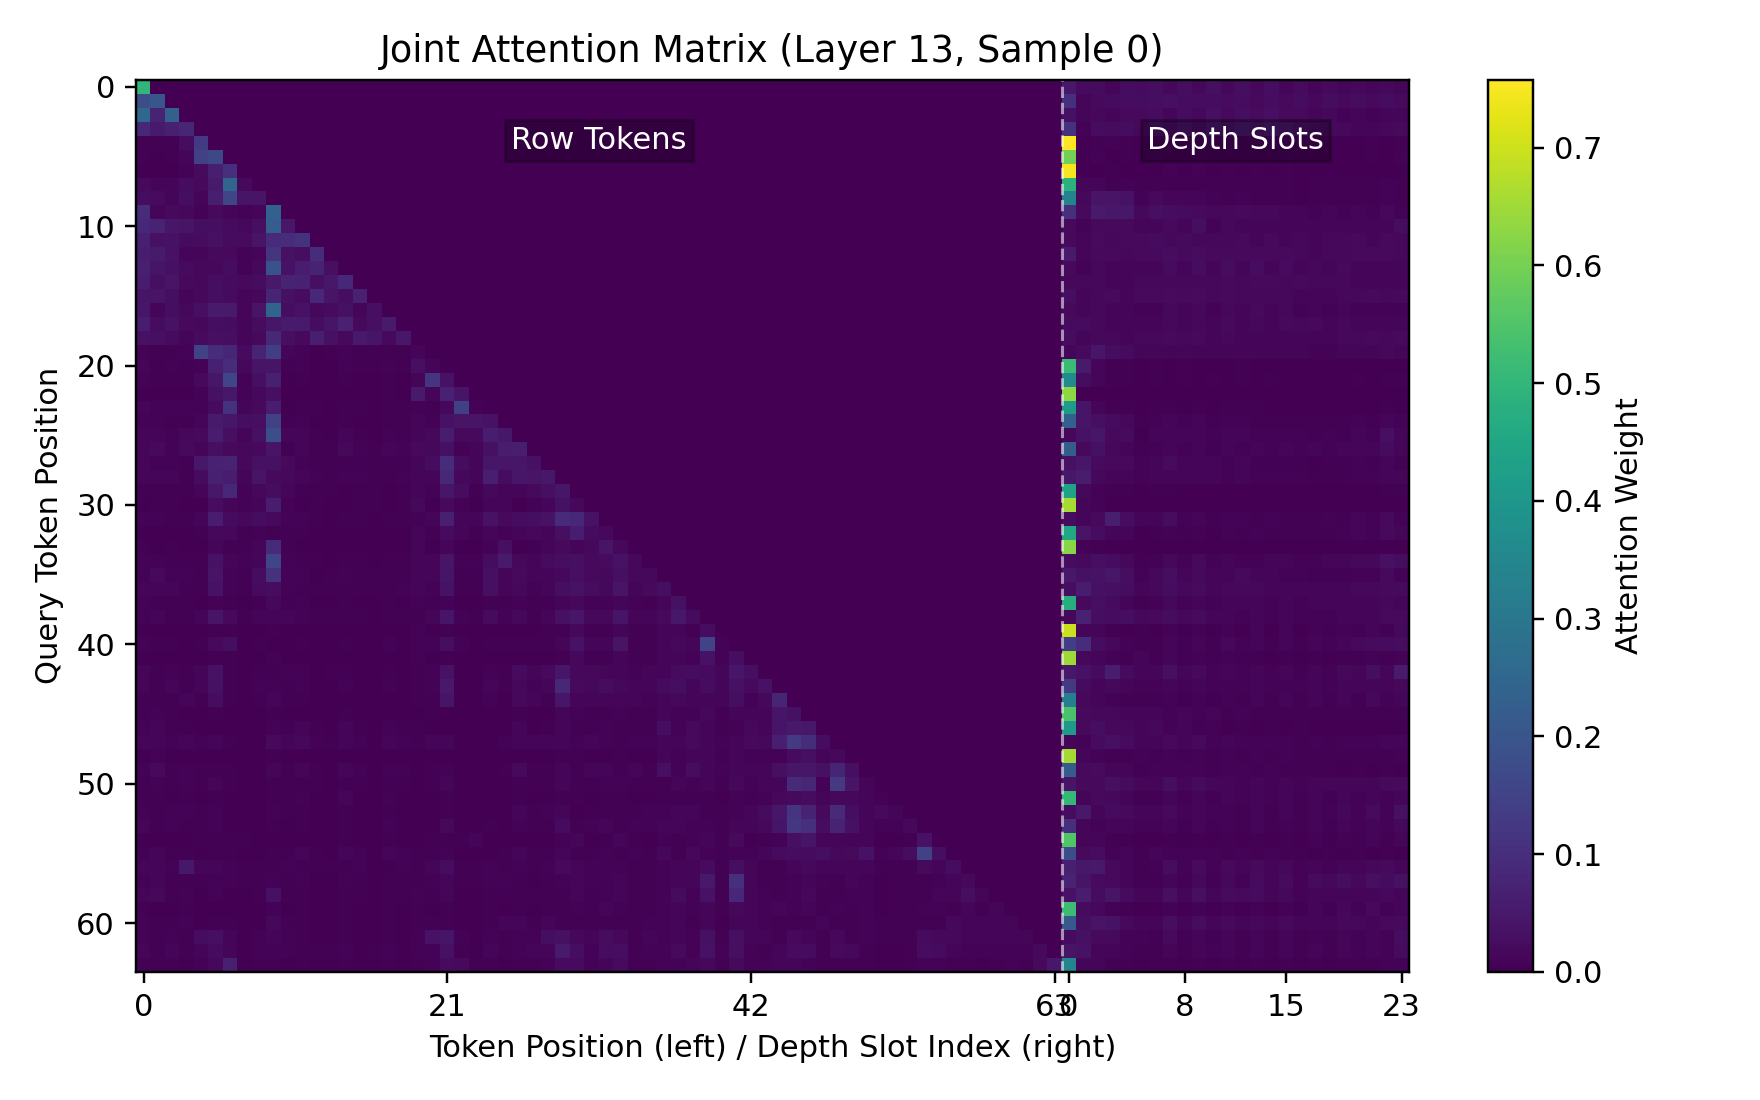
\includegraphics[width=0.48\linewidth]{figures/figure3d_ours_joint_attention_s64.png}
    \caption{Attention-allocation analysis. Top left: average row-vs-depth attention mass by layer, showing that the depth branch becomes substantially more active in middle and late layers. Top right: depth-memory slot heatmap, showing that retrieval is selective rather than uniformly spread over all historical slots. Bottom left: baseline attention matrix ($seq=64$, layer 13), where all mass is distributed over token positions only. Bottom right: proposed joint attention matrix ($seq=64$, layer 13), where part of the attention budget is routed to a distinct region of layer-depth slots.}
    \label{fig:attention-analysis}
\end{figure}

\section{Related Work}

Modern decoder-only language models are built around causal self-attention over the token dimension. This design has proved extremely effective, and prior work has long emphasized that one of its key benefits is the drastic reduction of communication path length along the sequence axis compared with recurrent architectures. Our work starts from the observation that this leaves a complementary axis underexploited, namely the depth history of the same token across previous layers.

A broad family of prior work has explored augmenting Transformers with memory mechanisms, recurrent state, cached history, or cross-layer interactions. Some methods enlarge the effective context window by storing additional information across segments or decoding steps; others revisit how later layers can reuse earlier representations more directly. Our method belongs most naturally to this second category, but with a narrower and more specific design goal: enabling a token at the current layer to retrieve its own same-position history from earlier layers and sublayers.

Another nearby line of work asks whether standard residual propagation can be improved by learned aggregation across layers. These methods are highly relevant to our motivation, since they also recognize that useful information may be distributed across depth rather than only along the current layer's token axis. However, our approach preserves the standard token-attention branch and organizes retrieval around same-position historical memory entries, rather than treating the entire layer stack as a generic pool for residual recombination.

\section{Conclusion}

This paper studies a simple architectural question: can a decoder-only Transformer benefit from explicitly reading the same token's depth history, rather than relying only on residual propagation through the layer stack? The experiments presented here suggest that the answer is yes. Across the completed WikiText-103 settings, a layer-depth memory routing mechanism yields stable perplexity improvements over standard Transformer baselines across multiple depths, sequence lengths, and training budgets.

The main empirical message is not that the gains are dramatic, but that they are repeatable. This is important because the baseline models used here are already reasonably strong, and therefore the observed 2\% to 4\% improvements are better interpreted as stable architectural gains than as artifacts of a weak comparison point.

At the same time, the work also exposes a clear trade-off. The current prototype incurs noticeable runtime overhead, and the measured slowdown is larger than the pure analytical compute increase. This indicates that the present implementation should still be viewed as an early but credible systems prototype rather than a fully optimized final design.

The broader conclusion is that depth history is a real information source for decoder-only language models. A token does not only need access to earlier tokens; it can also benefit from direct access to what earlier layers already computed at the same position. The accompanying attention analyses support this interpretation: the trained model assigns substantial mass to the depth branch in deeper layers and concentrates retrieval on a small number of high-value historical slots rather than ignoring the branch or averaging uniformly over history. The proposed layer-depth routing mechanism provides one concrete way to expose that signal. Future work should further clarify the best memory parametrization, improve runtime efficiency, and test whether the same design principle scales to larger models and broader language-model settings.

\end{document}
